% *********************************************************************
% © 2010–2026 Jeremy Sylvestre
%
% Permission is granted to copy, distribute and/or modify this document
% under the terms of the GNU Free Documentation License, Version 1.3 or
% any later version published by the Free Software Foundation; with no
% Invariant Sections, no Front-Cover Texts, and no Back-Cover Texts. A
% copy of the license is included in the appendix entitled “GNU Free
% Documentation License” that appears in the output document of this
% PreTeXt source code. All trademarks™ are the registered® marks of
% their respective owners.
%
% *********************************************************************

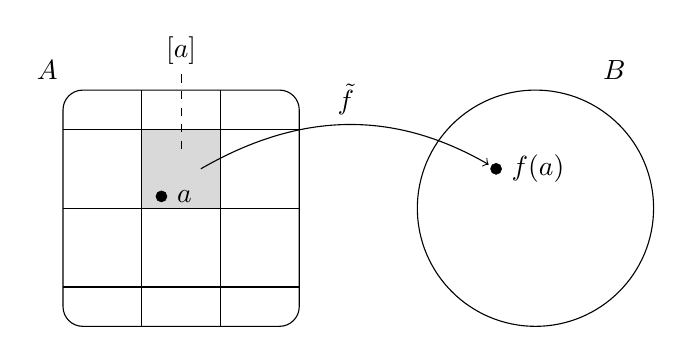
\begin{tikzpicture}[
	vertex/.style={ circle, draw, very thin, fill, inner sep=0pt, minimum size=4pt },
	vertexg/.style={ black!40!white, circle, draw, very thin, fill, inner sep=0pt, minimum size=4pt },
	vertexo/.style={ circle, draw, very thin, inner sep=0pt, minimum size=4pt }
]

\fill[black!15!white] (-3,0) -- (-2,0) -- (-2,1) -- (-3,1) -- (-3,0);
\draw (-3.5,1.5) -- (-3.75,1.5)
	arc (90:180:0.25cm) -- (-4,-1.25)
	arc (180:270:0.25cm) -- (-1.25,-1.5)
	arc (270:360:0.25cm) -- (-1,1.25)
	arc (0:90:0.25cm) -- (-3.5,1.5);
\node at (-4.2,1.75) {$A$};
\foreach \l in {-3,-2}
	\draw (\l,1.5) -- (\l,-1.5);
\foreach \l in {-1,0,1}
	\draw (-4,\l) -- (-1,\l);
\node at (-2.5,2) (a) {$[a]$};
\draw[dashed] (a.south) -- (-2.5,0.75);
\draw (2,0) circle (1.5cm);
\node at (3,1.75) {$B$};
\node at (1.5,0.5) (y) [vertex,label=right:{$f(a)$}] {};
\node at (-2.75,0.15) (x) [vertex,label=right:{$a$}] {};
\draw[->,shorten >=1pt] (-2.25,0.5) to [out=30,in=150] node[above] {$\tilde{f}$} (y);

\end{tikzpicture}
